\documentclass[11pt,letterpaper,english]{article}
\usepackage[T1]{fontenc} % Standard package for selecting font encodings
\usepackage{txfonts} % makes spacing between characters space correctly
\usepackage{xcolor} % Driver-independent color extensions for LaTeX and pdfLaTeX.
\usepackage{hyperref}  %The ability to create hyperlinks within the document
%\usepackage{blindtext} % To create text
%\usepackage{mdwlist} % mdwlist for compact enumeration/list items
%\usepackage[pagestyles]{titlesec} % related with sections—namely titles, headers and contents
\usepackage{fancyhdr} % header footer placement

\usepackage[top=1in, bottom=1in, left=1in, right=1in] {geometry} % Margins
\usepackage{graphicx}   % Essential for adding images to you document.

\usepackage{enumitem}  % Helps with the reduce itemize/enumerate separations

\usepackage{sectsty}
\sectionfont{\normalsize}
\subsectionfont{\normalsize}
\subsubsectionfont{\normalsize \it}

\usepackage[font=bf]{caption}
\captionsetup{labelsep=period}

\setlength{\parskip}{\baselineskip}%
\setlength{\parindent}{0pt}%


\pagestyle{fancy} % allows you to use the header and footer commands


\raggedright
\begin{document}

\setlength{\parindent}{0in} % Amount of indentation at the first line of a paragraph.

\pagestyle{fancy} \lhead{The Detailed Physical Structure of the Circumgalactic Medium} \rhead{Evan Schneider} \renewcommand{%
\headrulewidth}{0.0pt}

\begin{center}
{\bf PROJECT NARRATIVE (The narrative should not exceed 15 pages)} 
\end{center}

\vspace{-.15in}

%\colorbox{yellow} {\bf {\emph{[Refer to the guidelines for additional instructions for preparing the proposal.]}}}

%\vspace{.15in}

%Visual materials, such as charts, graphs, pictures, etc., are included in the 15-page limit. References {\bf do not} count in the 15-page limit and should be listed after the Project Narrative. URLs that provide information related to the proposal should not be included. {\bf The 15-page limit will be strictly enforced.}  The Project Narrative should address the following points:

\vspace{-.25in}
\section{SIGNIFICANCE OF RESEARCH}
\vspace{-.2in}
%List any previous INCITE award(s) received and discuss the relationship to the work proposed. Explain what advances you expect to be enabled by an INCITE award that justifies an allocation of petascale resources (e.g., anticipated impact on community paradigms, valuable insights into or solving a long-standing challenge, etc.). Place the proposed research in the context of competing work in your discipline or business. The information should be sufficient for peer review in your area of research and also appropriate for general scientific review comparing your proposal with proposals in other disciplines. Potential scientific or business impact is the predominant determinant for awards. This factor will be assessed by a peer-review panel. Also list any previous INCITE award(s) received and discuss the relationship to the work proposed. {\bf This section is typically about 4 pages.}

%When you cite a reference, please insert a number in brackets, as shown here [1], to correspond to its number on the reference list at the end of this template. Please call out the references in numerical order and list them in the same way. The reference list will {\bf not} count toward the 15-page limit.
%(Placeholder text. This section should be about {\bf 1 page}.)

%This first section should be broad enough for a general audience comparing our proposal with those in other disciplines.

%Broad science overview paragraph, including bold (literally and figuratively) thesis statement.

%Brief statement of the problem.

%Brief description of the proposed simulations (solution).

%Brief description of the impact of the project on the community.

%(Brief description of previous awards and their relation to this proposal.)

Large-scale simulations of galaxy formation in the universe have made enormous strides in the past decade, with models that are now able to reproduce a remarkably wide range of observations.  However, the ability of these models to make predictions is hampered by their inability to resolve the small-scale gas physics that regulates how baryons get into and out of galaxies in a physically self-consistent manner. Because of the enormous range of scales involved, these simulations must use ad-hoc recipes, known as "sub-grid models", to represent small-scale physical processes. These recipes are calibrated against observations, strongly reducing the ability of simulations to constrain fundamental physics such as the nature of dark energy or dark matter. Some of the most challenging sub-grid physical models involve the multi-phase gas in and around galaxies. In the past, such models could not be developed or tested through direct simulation due to the large range of scales present in multi-phase astrophysical flows; however, recent advances in hardware and software have now made it possible to carry out the numerical experiments required to understand these flows. {\bf This proposal lays out a systematic plan that harnesses the leadership computing facility Summit and our GPU-native hydrodynamical simulation code {\tt Cholla} \cite{Schneider15} in order to understand the development and evolution of multi-phase, turbulent astrophysical gas flows by resolving the relevant scales for the first time.}

Many astrophysical systems produce turbulent, pressure-confined diffuse gas which is prone to the development of thermal instabilities. Such systems include the interstellar medium (ISM) and circumgalactic medium (CGM) of galaxies, and even the intracluster medium (ICM) of high-mass galaxy clusters. Hence, the physics of thermally-unstable turbulent gas is likely to play a key role in the evolution of many systems. While the linear evolution of the thermal instability in extremely simplified systems has been well-studied, we still lack a good understanding of how this gas evolves in the non-linear stages and how the multi-phase state saturates. A wide range of scales is likely to be involved and yet the cold clouds that form will be widely distributed -- to simulate such a combination requires high resolution throughout the domain. We are particularly motivated by recent observations of the CGM, the diffuse gas which lies outside of the disk of the galaxy, fills its dark matter halo, and yet is still gravitationally bound to the overall system (which is dominated in mass by dark matter). While this gas emits radiation very faintly and is difficult to detect directly, recent studies using absorption lines in the spectra of bright background sources have been used to probe the CGM by measuring column densities of hydrogen and other elements. These observations have produced a theoretical challenge by detecting gas at a wide range of temperatures and ionization states, something that cosmological simulations conspicuously fail to reproduce or explain because they lack the resolution to model multiphase gas.

Here, we propose to carry out a set of simulations of a small region of the CGM (we focus on the CGM in this proposal, but we expect our results to be much more widely applicable).  As described in more detail below, we have identified both the smallest and the largest scales that we believe we need to simulate in order to develop a physical understanding of the dynamics of cooling, turbulent gas.  The requirements are severe, with a ratio of largest to smallest length scales of order $10^{3-4}$; moreover, because of the turbulent nature of the gas, the cold clumps which condense out can do so anywhere and at many places nearly simultaneously, with no preferred geometry.  This means that we simply need to simulate the entire region at high resolution, a requirement which has previously prevented this work from being done.  We will perform simulations to first determine the required resolution to numerically converge on the distribution of gas phases (our key takeaway), and then systematically vary the mean properties of the box (primarily pressure and velocity dispersion of the turbulent gas) in a manner informed by global-scale galaxy simulations. From these simulations, we will develop both a physical understanding of the multiphase gas as well as simple model that can be included in large-scale simulations.  In this way, we aim to make the cosmological simulations much less dependent on tuned sub-grid models and therefore more predictive.



\vspace{-.25in}
\subsection{Scientific Motivation}
\vspace{-.2in}

%(Placeholder text. This section should be about {\bf 2 pages}.)

%This is where we really dig in to the science. The level should be appropriate for peer review in astrophysics.

%Outline the science background. I like to start with an interesting observation, followed by a problem, followed by our solution to the problem. Possible structure:
%\begin{itemize}
%\item{Background: recent observational studies of the CGM (COS and friends)}
%\item{Theoretical puzzle: how to explain the cool gas in galaxy halos? Observations point towards small-scale structures, well below the resolution limit of current cosmological simulations.}
%\item{Theoretical solution: small volume-filling cool structures seeded by turbulence + thermal instability in the CGM. Possibly very small - $c_\mathrm{s} t_\mathrm{cool}$ of order a few to tens of parsecs (see Figure~\ref{fig:cs_tcool}).}
%\item{Logical numerical study: simulations of patches of the CGM with driven turbulence and astrophysical cooling, with $c_\mathrm{s} t_\mathrm{cool}$ resolved. For driving scales of order 1 kpc, this will require very high resolution boxes.}
%\item{What will be gained from the study.}
%\item{Additional benefits to the community (e.g. better physical understanding of CGM phase structure to inform observations, subgrid model for cosmological simulations, etc..}
%\end{itemize}

The circumgalactic medium (CGM) plays a critical role in the modern picture of galaxy formation: gas first enters the CGM from the intergalactic medium, often via (possibly cold) filamentary flows and material stripped from merging halos; it accretes onto the star forming (disk) galaxy at the center of the halo, fueling star formation; and it receives ejected gas via stellar and black-hole feedback in the disk, often termed the galactic `fountain' (see \cite{Tumlinson17} and \cite{Putman12} for recent reviews of the CGM).  Much of the halo gas is likely to be shock-heated to nearly the virial temperature, and in approximate hydrostatic equilibrium (e.g., \cite{White78, Fielding17}. Substantial evidence for this hot gas exists \cite{Bregman07}, but cold and warm gas is also likely to co-exist in the halo (e.g., \cite{Keres09, Wakker2009, Rigby02}). Indeed, recent observations have demonstrated the presence of cold and possibly dense gas clouds in the outskirts of the CGM \cite{Tumlinson13, Werk14, Lau16}, with temperatures around $10^4$ K as well as warmer gas with intermediate, $T \sim 3 \times 10^5$ K temperatures \cite{Chen2009, Prochaska2011}.  Such multiphase gas has proved exceptionally difficult for cosmological simulations to reproduce, with theoretical predictions often under-predicting observations by several orders of magnitude \cite{Hummels2013}.  

Understanding the details of this multiphase medium has the potential to shed light on the fundamental processes regulating galaxy formation. In recent years rich data sets have been collected demonstrating a strong correlation between CGM properties and galaxy mass, star formation rate (SFR), redshift, and distance from galaxy \cite{Tumlinson11, Bordoloi14, Borthakur15}. These observations reflect the CGM's prominent role in determining how galaxies accrete, eject, and recycle their gas. One of the most puzzling findings of these studies is the high covering fraction of cold gas ($T\sim10^4$ K) -- traced by neutral hydrogen H\,\textsc{i} and singly ionized elements such as Mg\ \textsc{ii}, C\ \textsc{ii}, and Si\ \textsc{ii} -- out to large distances ($\gtrsim 100$ kpc) seemingly independent of galaxy properties \cite{Thom12}. These observations present an intriguing view of the rich structure 10s to 100s of kpc from galaxies but have remained difficult to model and interpret. The primary reason for this difficulty, demonstrated in Fig.\,\ref{fig:multiphase}, 
is the sensitivity---particularly at low temperatures---of the ions used as observational CGM tracers to small changes in the poorly understood phase structure. 
%Different ions are sensitive to different regions of the often poorly constrained phase distribution. 
\textit{A detailed understanding of what sets the gas distribution across the full range of temperatures is crucial for accurately interpreting the observations and using them to their full potential to constrain the properties of galaxy halos and the galaxies residing within them.}


\begin{figure}[t]
    \centering
    \begin{minipage}{0.6\textwidth}
        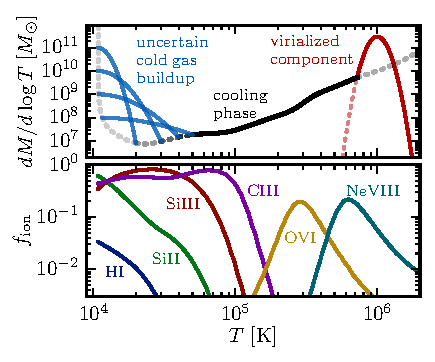
\includegraphics[width=\textwidth]{../figures/dMdlogT_picture_ion_all_P100_broad_narrow_3in.pdf} 
    \end{minipage}\hfill
    \begin{minipage}{0.4\textwidth}
        \centering
\caption{\textit{Top}: Phase distribution showing the contribution from the virialized, cooling, and cold components. The sensitivity of the coldest phase to resolution and microphysics lead to changes in its distribution. \textit{Bottom}: Ion fraction for various ions that are or can be observed in the CGM of low redshift galaxies assuming they are at a pressure of $P/k_B = 100\,\mathrm{K\,cm}^{-3}$. Small changes to the phase structure at low temperatures can have a major impact on the observed ion column densities and therefore the inferred CGM properties.\label{fig:multiphase}} 
\end{minipage}
\end{figure}

%Because the CGM is extremely dilute and can only be detected in absorption when there is a chance alignment of a bright background source the observational picture is far from complete. Nevertheless, these discrete pencil-beam windows into the properties of the halo gas can be illuminating. These observations typically yield a measurement of the amount of a given ion along the line of sight, quantified by the column density $N_{\rm ion} = \int n_{\rm ion} ds$, as well as the velocity of the absorbing gas. In recent years much work has been devoted to measuring how these properties relate to the property of the host galaxy. These observational studies have demonstrated a close relationship between key galactic properties such as stellar mass and star formation rate and the properties of the CGM [cite] highlighting the integral role of the CGM in galaxy formation. 

There is reason to believe that the cold phase of the CGM resides primarily in small clumps ($\ll 1$ kpc).  From an observational stand point, this is supported by the fact that cold gas properties are seen to vary on sub-kpc scales
% in close quasar pairs and gravitationally lensed quasars 
 \cite{Rauch02, Churchill03, Lopez18}, and that photoionization models favor high volume densities \cite{Werk14,Lau16}. On the theoretical side, both analytic arguments and simple numerical experiments indicate that thermal instability saturates to a state in which cold clouds embedded within a static hot medium have a characteristic size $\ell_{\rm cool} = c_{\rm s}\, t_{\rm cool}$ that is set by the pressure of the confining medium \cite{McCourt18}, as shown in Fig. \ref{fig:cs_tcool}. Here $\ell_{\rm cool}$ is the length scale of the cloud, $c_{\rm s}$ is the sound speed in the cooled gas, and $t_{\rm cool}$ is the cooling time of the gas -- the total energy divided by the rate at which energy is lost due to radiative processes. Physically, this scale can be understood as the maximum size a cloud can have while still maintaining pressure equilibrium with its environment. 



%The high observed occurrence rate of cold gas at large radii in galactic halos presents a difficult theoretical challenge. There is indirect evidence that the cold gas being probed by these observations resides in clouds vastly smaller than can be resolved in the even the most cutting-edge high resolution cosmological simulations. Much of this evidence is derived by comparing the observed column density of an ion to a model for its volume density the ratio of which yields a characteristic spatial scale $\ell = N/n$ usually on the order of a few tens of pc. Additionally, rare close pairs or gravitationally lensed multiply imaged of background sources also show sizable differences on scales on the order of a kpc or less. 

%There is, in fact, a theoretical reason to believe that cold gas should reside in small clouds. As an over dense region in the CGM begins to cool out of the ambient hot medium the gas will try to maintain pressure equilibrium. Pressure equilibrium can only be maintained if the sound crossing time, $r_{\rm cloud}/c_{\rm s}$ the time on which pressure is readjusted, is less than the cooling time $t_{\rm cool}$. Therefore as the region cools it will break up into smaller and smaller clouds that maintain this balance of time scales. Eventually as the gas approaches the temperature where cooling becomes inefficient the cooling time increases and breaking up any smaller is no longer beneficial to maintaining pressure equilibrium. The clouds therefore will reach a characteristic size scale roughly equal to the minimum of value of $c_{\rm s}\, t_{\rm cool}$ for the pressure of the confining hot medium, which we refer to as $\ell_{\rm cool}$ \cite{McCourt18}. This length scale ranges from a kpc at low pressures to a fraction of a pc at small scales. 

\begin{figure}[ht]
    \centering
    \begin{minipage}{0.425\textwidth}
	\caption{ The bottom panel shows the largest and smallest relevant length scales as a function of pressure. The dark blue line shows $\ell_{\rm cool} = c_{\rm s} \, t_{\rm cool}$, which is the expected characteristic cold cloud size \cite{McCourt18}. The orange dashed line traces $R_{\rm CGM}$, the characteristic radius in the CGM at a given pressure from global CGM simulations \cite{Fielding17}, which is roughly the turbulent driving scale. The top panel shows the ratio of these length scales, which corresponds to the minimum number of resolution elements required in one direction to reach $\Delta x = \ell_{\rm cool}$. The stars show the value at the pressure of our target simulations. \label{fig:cs_tcool}}
    \end{minipage}\hfill
    \begin{minipage}{0.575\textwidth}
        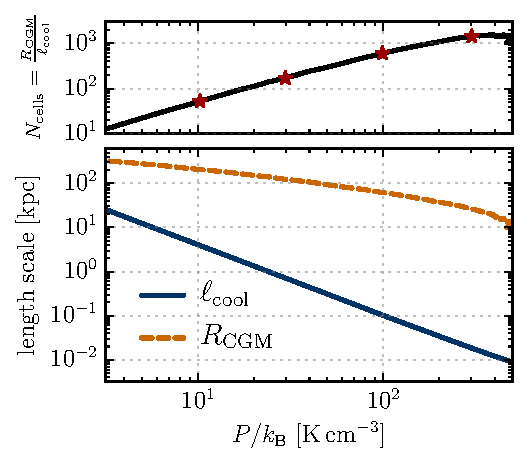
\includegraphics[width=\textwidth]{length_scales_sim.pdf} 
    \end{minipage}
\end{figure}

The small expected sizes of these clumps may explain the observed order unity cold gas covering fraction, because for fixed cold gas mass a large number of small clouds has a higher covering fraction than a small number of large clouds. Additionally, small clouds can be more easily entrained by the hot medium due to their small surface area to volume ratio. Efficient entrainment would prevent the clouds from immediately "raining out" of the CGM due to their reduced buoyancy. Estimates of the implied accretion rate onto the galaxies if the cold gas does rain out is orders of magnitude larger than the observed star formation rate and would, as a result, require vast amounts of heating \cite{McQuinnWerk}. This is particularly problematic in the case of the cold gas observed around quiescent galaxies. This difficulty is mollified if the cold gas is instead long lived and stays roughly where it formed due to efficient entrainment, a natural result of cooling out of the hot phase.

To account for the large observed covering fraction of cold gas in the CGM these small cold clouds must grow throughout the halo. Moreover, because the present day star formation rates are significantly less than the accretion rates into the CGM from the IGM the bulk of the CGM must be quasi-static. Therefore, the cooling that leads to the development of the cold clouds must be balanced by some form of heating. Turbulence in the CGM provides a natural explanation to both of these problems. The compressive modes of a turbulent flow lead to density enhancements and the dissipation of the turbulent kinetic energy can offset cooling. Moreover, CGM turbulence is observed via the broad line widths in  absorption spectra and expected theoretically to be driven by the winds emanating from galaxies and from the stirring by satellite galaxies. 

Controlled global-scale simulations of the CGM (carried out by co-PI Fielding) have shown that kinetic energy injected by galactic winds and the subsequent turbulent dissipation heating can sufficiently limit halo cooling \cite{Fielding17}. 
The resulting halos are roughly hydrostatic and the star formation rates are dramatically reduced relative to intergalactic accretion rates. 
The phase structure (and, as a result, the mock observations) demonstrated a marked dependence on the pressure (set by the location in the halo and the dark matter halo mass) and the velocity dispersion (related to the strength of the galactic feedback). 
This reflects the competition between cooling (pressure-dependent) and turbulent mixing (velocity-dependent) in determining the phase balance.
{\em Although these models successfully explain many of the bulk CGM properties, the low temperature end of the phase structure never converged numerically even when the resolution was pushed to $\sim 100$ pc---the highest resolution global scale CGM simulation to date}. 

We propose to study the turbulent thermal instability in the CGM at unprecedented resolution. The range of scales in this problem is challenging because it is necessary to resolve both the large-scale turbulent properties and the small-scale cold clouds. Fig. \ref{fig:cs_tcool} shows the expected range of scales for a range of pressures relevant to the CGM (and to the ICM and ISM in some limits). Turbulence is driven on large scales roughly equal to size of the region, so for a given pressure we estimate the driving scale to be (a fraction of) the radius of the CGM that has that characteristic pressure. This varies from a few hundred kpc for the lowest pressures at the outskirts of the halo to roughly 10 kpc in the high pressure inner halo. To accurately model the cold phase we must resolve $\ell_{\rm cool}$, which scales more strongly with pressure than the turbulent driving scale. In the inner CGM this leads to a range of scales of $\sim10^3$, while in the outer halo the requirements are less stringent.

These simulations will for the first time model the full phase structure of the CGM in a fully resolved sense. This will have major implications for the interpretation of ever growing body of observations and will unlock the potential of using the CGM as a probe of fundamental galaxy formation physics. Furthermore, given the potential impact of multiphase cooling on the dynamics and evolution of halo gas, these simulations will provide the ideal basis to develop a sub-grid model for the unresolved CGM phases in global scale cosmological simulations, as has been used for the ISM for decades \cite{SpringelHernquist}.




\vspace{-.25in}
\subsection{Results from Previous INCITE Awards and Relation to Current Proposal}
\vspace{-.2in}

%(Placeholder text. This section should be {\bf < 1 page}.)

Our early awards on LCF systems were associated with developing the {\tt Cholla} software that enables this proposal. These previous awards include DD projects AST107 "Scaling the GPU-enabled Hydrodynamics Code {\tt Cholla} to the Power of Titan" and AST119 "Extending the Physics of the GPU-Enabled {\tt Cholla} Code to the Power of Titan". PI Schneider was a co-I on both of these awards and is the primary architect of the {\tt Cholla} code. Results from project AST107 included the first demonstration of {\tt Cholla} at petascale. AST119 allowed the development of further physics modules, including the GPU-accelerated radiative cooling that will be crucial to the simulations described in this proposal. As a practical application for project AST119, we investigated the cloud-wind problem, which is directly related to the puzzling observations that motivated this proposal. In that work, we demonstrated that the presence of $10^4$ K gas in the CGM cannot be directly explained by ram pressure acceleration of dense disk material within a hot, supernova-driven wind, therefore requiring an origin for this gas that involves thermal instability \cite{Schneider17}.

PI Schneider is also the co-PI of the ongoing INCITE project AST125 "Revealing the Physics of Galactic Winds with Petascale GPU Simulations". This project has produced the most detailed numerical models of multiphase galactic winds ever, a system that is also closely related to the work considered in this proposal \cite{Schneider18a}. These high resolution simulations have demonstrated that thermal instability in winds can be a source of cool gas that could reach the CGM \cite{Schneider18b}. However, the increased pressure in these winds meant that even stricter resolution requirements were required than for our proposed CGM simulations. As a result, the wind simulations carried out as part of AST125 only extend to $R_{\rm CGM} = 10$ kpc, and thus cannot be used to determine what happens to the gas in the wind once it travels beyond this radius. Also relevant to this proposal, these simulations have shown that starburst winds can be a major driver of the large-scale turbulence that is the primary source of energy for our proposed CGM simulations (see also \cite{Fielding17}).


\vspace{-.25in}
\section{RESEARCH OBJECTIVES AND MILESTONES }  
\vspace{-.2in}
%Describe the proposed research, including its goals and milestones and the theoretical and computational methods it employs. Goals and milestones should articulate simulation and developmental objectives and be sufficiently detailed to assess the progress of the project for each year of any allocation granted. Milestones should correlate with those in the milestone table. It is especially important that you provide clear connections between the project's overarching milestones, the planned computational campaign, and the compute time expected to be required for this campaign (e.g., should correlate with those in the ``Use of Resources Requested''). {\bf This section is typically about 6 pages.}

%(Placeholder text. This section should be about {\bf 6 pages}.)

%This section needs a lot of filling out. Basically, this is where we describe the set of simulations we plan to do, and why we're doing them. I've come up with a baseline set of simulations that I think we could do based on the computational time, and a baseline set of objectives and milestones. In describing the simulations, we should include density and temperature projections (I've put some that I generated in as placeholders at the moment). I think some of Drummond's density / temperature pdfs would be good in this section as well, to help describe the analysis we will do and how it relates to our research objectives.

As the discussion in the previous section makes clear, understanding the phase structure of turbulent, pressurized astrophysical flows is key to modeling galaxies. However, adequately resolving this structure is computationally challenging, with the ratio of the energy injection scale to the cooling length of order $R_{\rm CGM}/\ell_{\rm cool} \approx 10^3$.  In this section, we describe a systematic plan to model these flows with conditions appropriate for a range of physical systems. First, we need to determine what resolution is required to converge on the properties of interest (object RO.A in Table~\ref{table:RO}).  As detailed earlier, we believe we know what range of scales are important, but it is not clear exactly how many cells across the cooling length $l_{\rm cool}$ are necessary to see convergence in the phase structure of the gas, nor do we know precisely how sensitive the results are to the largest scales modeled ($R_{\rm CGM}$).  Therefore, to begin, we will develop a fiducial simulation (with parameters typical of the Milky Way CGM) and carry out a convergence study.  Once the convergence requirements are set, we will systematically vary our key parameters---the velocity dispersion and mean pressure in the box---in order to develop an understanding of the physical state of thermally unstable turbulent flows for a variety of environments (RO.B). Finally, we will use these results to connect back to the global galaxy simulations (and their cosmological cousins) by developing a simple physical model and generating observational predictions (RO.C and RO.D). We more fully outline the proposed project milestones (see Table~\ref{table:RM}) and their connections to these objectives in the following subsections.


\begin{table}[h]
%\centering
%\vspace{-.12in}
\caption{Research Objectives}
\label{table:RO}
\begin{tabular}{|l|p{5.8in}|}
%\multicolumn{2}{l}{\bf{Table 1: Research Objectives}}\\
\hline
\textbf{RO.A} & Determine the effects of numerical resolution on current attempts to characterize the CGM. \\ \hline
\textbf{RO.B} & Describe the physical nature (phase structure, cloud sizes, velocity coherence length etc.)
of gas in thermally unstable flows as a function of turbulent mach number and pressure. \\ \hline
\textbf{RO.C} & Develop a model that characterizes the unresolved CGM across a range of
pressures and mach numbers for implementation in cosmological simulations. \\ \hline
\textbf{RO.D} & Identify relationships between the physical state of the CGM and other relevant galaxy
properties, both simulated and observable (e.g. halo mass, star-formation rate, etc.). \\
\hline
\end{tabular}
\end{table}

\begin{table}[h]
%\centering
%\vspace{-.12in}
\caption{Research Milestones}
\label{table:RM}
\begin{tabular}{|l|p{4.7in}|p{0.9in}|l|} 
%\multicolumn{3}{l}{\bf{Table 2: Research Milestones}}\\
\hline
\multicolumn{2}{|l|}{\bf Milestone} & {\bf Objective} \\ \hline
\multicolumn{3}{|c|}{\it Semester 1} \\ \hline
\textbf{RM.A} & Develop fiducial turbulent CGM model and run convergence study, including first petascale simulation of the CGM. & RO.A , RO.B \\ \hline
\multicolumn{3}{|c|}{\it Semester 2} \\ \hline
\textbf{RM.B} & Parameter study: Run suite of turbulent box simulations at varying velocity dispersion and CGM pressure. & RO.B, RO.C\\ \hline
\textbf{RM.C} & Compute ionization fractions for various species using results of all simulations for comparison with observational surveys of the CGM. & RO.D \\ \hline
\end{tabular}
\end{table}

\vspace{-.25in}
\subsection{RM.A: A Numerically Converged Model of the Milky Way CGM}
\vspace{-.2in}

Due to our location within it, the Milky Way is the galaxy with the best-observed circumgalactic medium, and therefore provides the best single system with which to compare the results of our simulation campaign. The Milky Way is also a fairly typical galaxy in the local Universe, with a dark matter halo mass $M \sim 10^{12}\,M_\odot$ near the knee of the galaxy mass function at present day. Its CGM pressure is likely to vary over the range of interesting pressures we will study, from the lowest potential pressures in the outer regions of the halo (P = 10), to the highest pressures in the inner halo (P = 300). Hence, Milky Way-like parameters are a logical choice for our fiducial model of the CGM and associated convergence study.

As described in Section 1, turbulent stirring in the CGM is likely a result of large-scale processes, such as galactic outflows. These processes inject energy on scales that may be an appreciable fraction of the characteristic CGM radius at a given pressure, $R_\mathrm{CGM} \sim 50 kpc$ for intermediate pressure regions of Milky Way. This driving scale sets the size requirement for our fiducial simulation box, with side lengths of $L_\mathrm{box} = 51.2\,\mathrm{kpc}$. Meanwhile, our best observational constraints on the Milky Way's CGM indicate that its pressure at intermediate radii ($R \sim 0.5 R_\mathrm{vir}$) is $P/k_\mathrm{B} \sim 100\,\mathrm{K}\,\mathrm{cm}^{-3}$. In Figure~\ref{fig:cs_tcool}, we showed that the relevant length scale for the pressure-confined, thermally-unstable cool clouds at this pressure is of order 100 parsecs. To demonstrate convergence of the properties of the CGM for this fiducial case will thus require a simulation with the ability to resolve this scale with an order of magnitude, while covering nearly three orders of magnitude in total dynamic range. (We estimate that ~8 cells are required to adequately resolve gas that is cooling as a result of thermal instability.) %Would be great to have a reference / justification for this. When it was 4 we had the Truelove criterion for gravity or the Koyama & Inutsuka 04 Field criterion for conduction ...

In Semester 1 of our project, we propose to carry out a convergence study of the properties of this fiducial model by simulating a turbulent box 51.2 kpc on a side, with progressively increasing resolution. These simulations will range from our lowest-resolution tests with $128^3$ cells ($\Delta x = 400\,\mathrm{pc}$), which are similar to the CGM resolution of a typical isolated galaxy simulation, to the highest resolution simulation with $8192^3$ cells ($\Delta x = 6.25\,\mathrm{pc}$). This highest resolution will be sufficient to demonstrate convergence down to a cool cloud scale of $100\,\mathrm{pc}$ if the clouds must be resolved by 8 cells (100 pc / 6.25 pc = the 16 cells required to see convergence). In addition to providing valuable scientific insight, this simulation will also carry its own significance as the first petascale simulation of the circumgalactic medium.

Figure~\ref{fig:CGMpatch} shows a density and temperature slice through a low-resolution test calculation that demonstrates our fiducial setup. In this simulation, turbulence is driven on large scales at wave numbers $1 \leq k L_{\rm box}/ 2 \pi \leq 2$. Energy is injected at each time step, at a rate set to balance the total energy that is radiated away by the cooling gas (see Section 3.4 for more information about our turbulent driving). As density inhomogeneities develop, the denser gas radiates away thermal energy more quickly, while the tendency towards maintaining pressure balance between phases compresses these clumps to even higher densities, fueling the instability. The result is a rich temperature and density structure characterized by many small clouds of dense gas entrained within a hot, turbulent medium.

\begin{figure}[t]
 \centering
 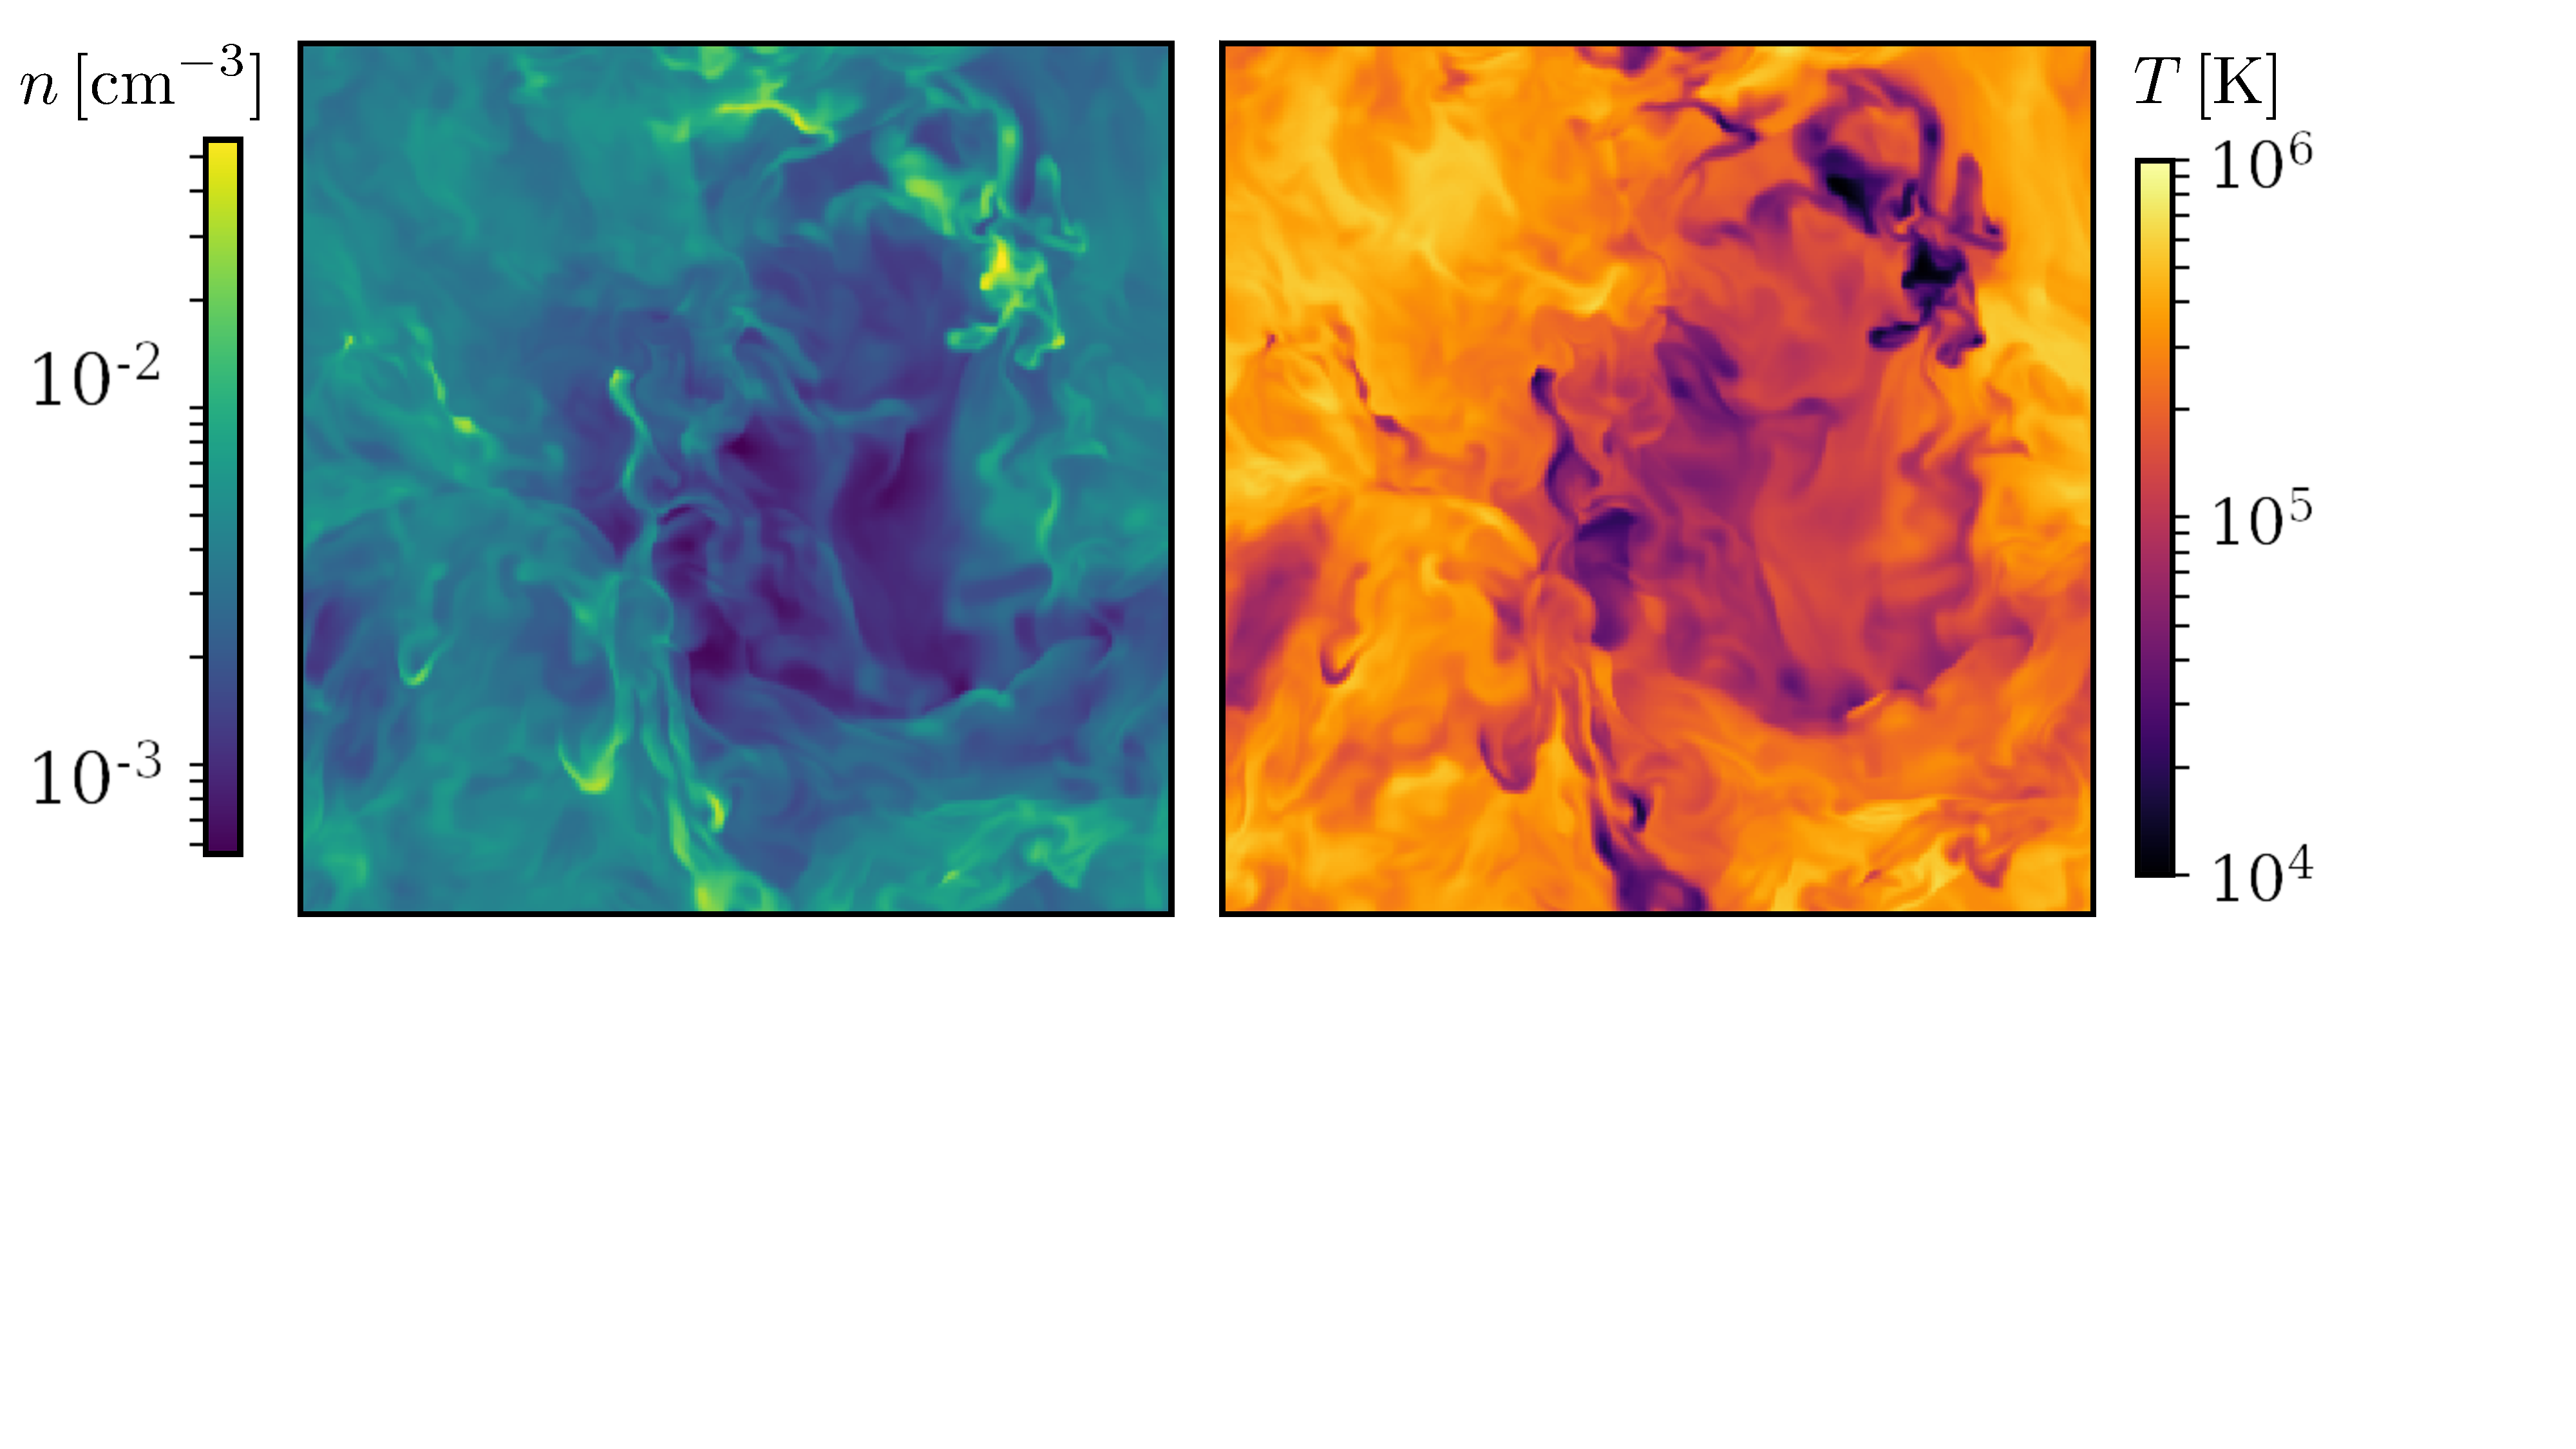
\includegraphics[width=1.0\textwidth]{Denstiy_Temperature.pdf} 
\caption{Two dimensional slices through a preliminary three dimensional local simulation showing the number density (left) and temperature (right) of a small patch of CGM. This simulation demonstrates the rich multiphase structure that develops via turbulence and thermal instability on scales well below what is obtainable with cosmological simulations. Accounting for this unresolved structure will bring global simulations into agreement with observations. \label{fig:CGMpatch}}
\end{figure}

%\begin{figure}[h]
%    \centering
%    \begin{minipage}{0.33\textwidth}
%        \centering\vspace*{-.25cm}
%\caption{Two dimensional slice through a preliminary three dimensional local simulation showing the temperature of a small patch of CGM with a representative average density, temperature, and velocity field. This 1 kpc per side simulation demonstrates the rich multiphase structure that develops via turbulence and thermal instability on scales well below what is obtainable with cosmological zoom-in simulations. Accounting for this unresolved structure will bring global CGM simulations \cite{Fielding17} into agreement with observations. \label{fig:CGMpatch}}
%    \end{minipage}\hfill
%    \begin{minipage}{0.67\textwidth}
%       \hspace{0.3cm} 
%        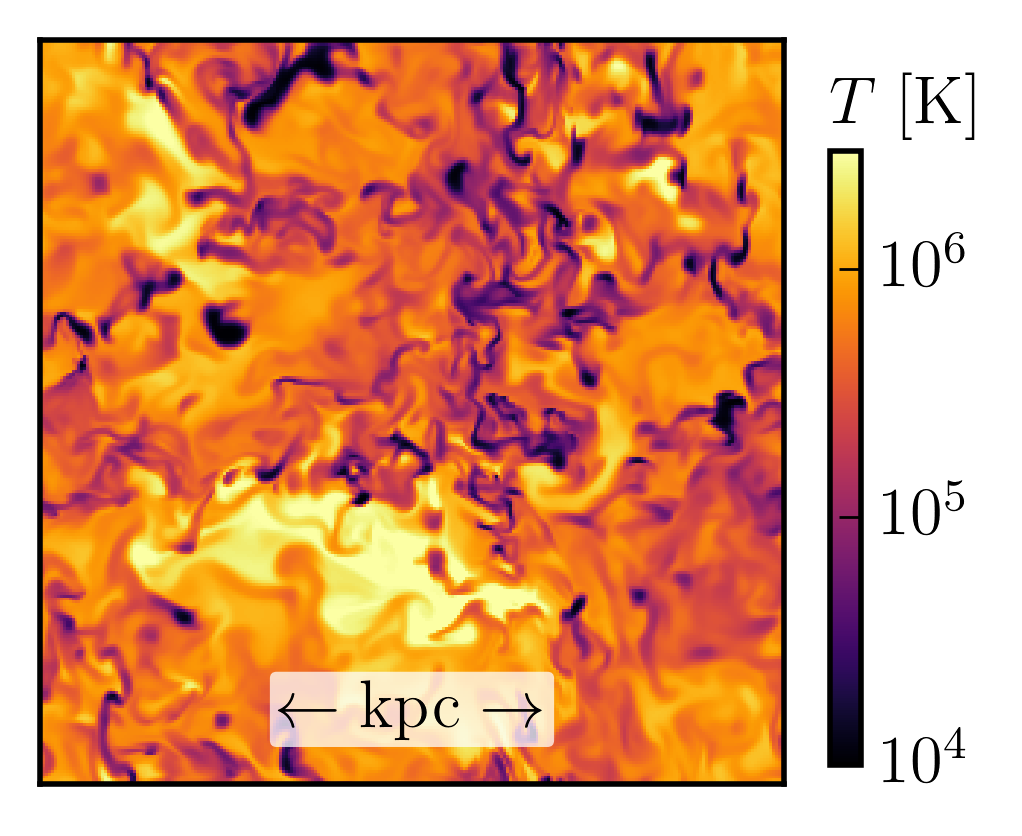
\includegraphics[width=1.04\textwidth]{T_proposal.png} 
%    \end{minipage}
%\end{figure}

In Figure~\ref{fig:sim_phase}, we show the distribution of mass as a function of temperature in this simulation at four different times. At early times ($t / t_\mathrm{cool} = 0.1$), the temperature distribution reflects the initial hot state, with a small spread in temperature as perturbations begin to develop. As time goes on and the simulation evolves, the thermal instability leads to a buildup of mass in the cooler phase. After roughly three cooling times, the simulation has reached an approximate equilibrium, as demonstrated by the shaded region around the $t / t_\mathrm{cool} = 3$ line, which shows the variation within $1\,t_\mathrm{cool}$ . We therefore determine that in order to adequately characterize the equilibrium state of the CGM gas in our simulations, we should run them for 3 cooling times of the initial hot phase. In the case of the Milky Way parameters shown here ($P/k_\mathrm{B} \sim 100\,\mathrm{K}\,\mathrm{cm}^{-3}$, $T = 3\times10^5$ K), $t_\mathrm{cool}$ for the hot gas is about 100 Myr.

\begin{figure}[t]
    \centering
    \begin{minipage}{0.5\textwidth}
        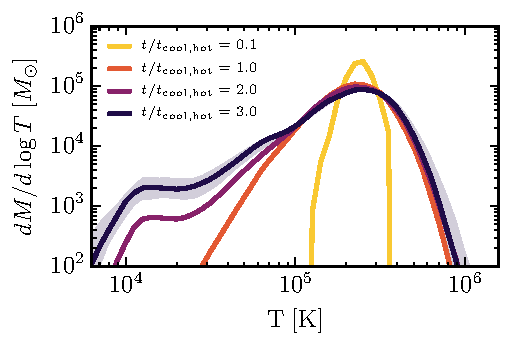
\includegraphics[width=1.\textwidth]{dMdlogT_proposal_t.pdf} 
    \end{minipage}\hfill
    \begin{minipage}{0.5\textwidth}
	\caption{  The amount of mass per logarithmic temperature bin $dM / d\log T$ from a preliminary turbulent thermal instability simulations shown at $t = 0.1,1,2,$ and $3$ times the cooling time of the hot phase, $t_{\rm cool,hot}$. The gray shaded region shows range during $ 2.5 \leq t / t_{\rm cool,hot} \leq 3.5$, which demonstrates the small variations around the steady state distribution. The final state has a cooling phase with $dM / d\log T \propto t_{\rm cool} \propto T^2$ between $3\times10^4$ and $3\times10^5$ K, as well as a pile-up at $T\sim10^4$ K. \label{fig:sim_phase}}
    \end{minipage}
\end{figure}


\vspace{-.25in}
\subsection{RM.B: How Velocity Dispersion and Pressure Affect the Phase Structure of the CGM}
\vspace{-.2in}



As demonstrated in low resolution idealized global simulations of the CGM, the turbulent mach number of the hot medium is not a constant function of radius (see Figure~\ref{fig:velocities}) \cite{Fielding17}. Typically, the processes driving turbulence (e.g. star formation feedback and winds) are most effective at small radii, leading to a distribution of mach numbers that peaks close to galaxies and falls off in the outer regions of halos (although we note that these are time and radially-averaged quantities, so there may be supersonic turbulent motions at large radii at discrete intervals). Moreover, these idealized simulations did not include satellite galaxies which can provide an additional source of turbulent stirring at large radii. Thus, in order to fully describe gas within the halo even of a single system with a given halo mass, we must simulate the CGM with a range of different velocity dispersions. Similarly, the pressure in the CGM varies as a function of both radius within the halo and total halo mass. To adequately characterize the full range of circumgalactic media that have been observed (and are relevant to cosmological simulations) will therefore require simulations across a range of CGM pressures, as well. Our second milestone will achieve this, as we carry out a parameter study across these two variables.

%Need to rework the following two paragraphs to reflect the parameters we've picked - M = 0.1, 0.5, 1; P = 10, 30, 100, 300 - and the fact that we will do a grid of simulations that span this parameter space. The three with P = 300 are expected to require $8192^3$ cells to be fully resolved, given $l = c_\mathrm{s} t_\mathrm{cool} \sim 10\,\mathrm{pc}$ and $R_\mathrm{CGM} ~\sim10\,\mathrm{kpc}$, so we will only do M = 0.1 and M = 1 for those. Not sure if any of what's below is useable.

Physically, the pressure determines the cooling time of the hot, volume-filling component since $t_{\rm cool, hot} \propto P^{-1}$. On the other hand the turbulent mach number regulates the width of the density distribution around the mean values. Higher turbulent mach number lead broader density distributions, which, therefore, will increase the amount of cool gas we expect to find populating the high density, low temperature, rapidly cooling tail of the distribution (see Figure~\ref{fig:sim_phase}). Turbulent motions, however, also tend to shred and destroy cold clouds as they condense out of the ambient medium. This competition between cooling and mixing is fundamental to the phase structure and overall dynamics, and yet has never been studied in detail. Our parameter survey will, for the first time, enable us to characterize how this competition plays out across the full range of spatial scales in different environments.

The range of pressures and mach numbers we will scan in our parameter study will cover the values predicted by idealized global CGM simulations \cite{Fielding17} and cosmological simulations \cite{Nelson+16}. We will run simulations with $P = 10, 30, 100$ and 300 K\,cm$^{-3}$.  At each pressure we will drive turbulence with mach numbers $\mathcal{M} = 0.3$ and 1, thereby probing the subsonic and transonic regimes. 
Based on the results of our convergence study (RM.A), we will know the number of grid cells per cold cloud size $\ell_{\rm cool}$ required to adequately resolve the phase structure of the gas.
The resolution at each pressure then be determined by the relation of the turbulent driving scale ($R_{\rm CGM}$) to the cold cloud size ($\ell_{\rm cool}$).
Figure~\ref{fig:cs_tcool} demonstrates that the resolution requirements are most stringent at high pressures. Preliminary testing indicates that $\lesssim 8 $ cells per $\ell_{\rm cool}$ is sufficient to achieve convergence. Working under this assumption, a $P=10$ K\,cm$^{-3}$ simulation with $512^3$ cells will fully resolve all scales, while at $P=300$ K\,cm$^{-3}$ $8192^3$ cells will be required to accurately model all scales. 

%The results of our convergence study (RM.A) will inform the number of cells per $\ell_{\rm cool}$ are necessary to adequately resolve the phase structure of the gas. 

%The first piece of our parameter study will focus on the effects of the turbulent mach number, as we run a series of simulations at fixed CGM pressure and scale the turbulent injection energy across the relevant range. In general, increasing the mach number of the turbulence will increase the width of the density pdf, and therefore will change the amount of cool gas we expect to find populating the high density / low temperature tail of the distribution . 

%Based on the results of our convergence study (RM.A), we will know what resolution is required to adequately resolve the phase structure of the gas. We will therefore be able to pick an appropriate pressure for this velocity dispersion study such that a set of moderate resolution simulations ($N = 4096^3$ cells) will be fully converged. Our initial anticipation is that this pressure will be similar to that of the Milky Way CGM, in which case we expect to be able to be able to characterize the CGM of our galaxy at a range of radii from the innermost halo out to the virial radius - a data set that will be invaluable for comparison to observations. Depending on the exact time step requirements (see Section 3.1), we anticipate carrying out 6 of these simulations in Quarter 2.


%Once we have developed an understanding of the effects of the velocity dispersion, we will turn to the pressure dependence of the CGM properties. As demonstrated in Figure~\ref{fig:cs_tcool}, we expect the pressure of the confining medium to be the primary factor that sets the length scale of the cool clouds embedded within it. To characterize this dependence, we will carry out a suite of simulations similar to those described in the previous paragraph, but this time at constant mach number while varying the pressure. Because the resolution requirement is expected to scale with the size of the cool clouds, the highest pressure simulations will also be the most computationally demanding, with CGM pressures of $P/k_B \sim 300$ likely requiring $N = 8192^3$ cells to be fully resolved. On the other hand, while the lower pressure simulations will have less strict resolution requirements, the lower average density of the gas will increase the associated cooling time ($t_\mathrm{cool} \propto n^{-2}$), while the physical time step set by the intermediate temperature gas remains the same, so these simulations will need to run for much longer in order for the phase structure to equilibrate. Both the high and low pressure simulations are thus expected to require petascale resources to be converged (see Section 3.1).



\begin{figure}[t]
    \centering
    \begin{minipage}{0.6\textwidth}
        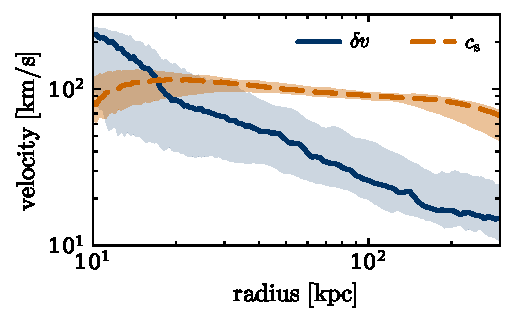
\includegraphics[width=\textwidth]{velocities.pdf} 
    \end{minipage}\hfill
    \begin{minipage}{0.4\textwidth}
        \centering
\caption{ Velocity dispersion (dark blue line; $\delta v = \sqrt{\langle v^2 \rangle - \langle v \rangle^2}$) and sound speed (orange dashed line; $c_{\rm s}$) profiles in global CGM simulations \cite{Fielding17}. The shaded regions trace the one sigma temporal variability around the median values over the full 9 Gyr duration of the simulation demonstrating the need to study how the phase structure changes for a range in Mach number $\mathcal{M} = \delta v /  c_{\rm s}$ from 0.1 to 1. \label{fig:velocities}} 
\end{minipage}
\end{figure}


\vspace{-.25in}
\subsection{RM.C: Connections to Cosmological Simulations and Observational Surveys}
\vspace{-.2in}

Much of the value of this project will be in the detailed analyses of these proposed simulations for comparison to cosmological simulations and CGM observations. With these simulations we will be able to precisely quantify the phase structure on scales unresolvable in cosmological simulations. This will enable us to develop sub-grid prescriptions for cosmological simulations to account for the unresolved cooling and dynamics. By doing so we will leverage the cosmological evolution and realistic environment that our simulations cannot include while still accounting for the crucial small scale dynamics. Sub-grid models have long been used to model the ISM of galaxies in such simulations \cite{SpringelHernquist} but no such model exists for the CGM despite its well established importance. 

From an observational standpoint, the goal is to constraint the physical state of the CGM (e.g., the pressure and Mach number) based on observations that measure the amount of a few ions along a line of site. Figure~\ref{fig:multiphase} demonstrates that different ions probe gas at different temperatures. Therefore, a detailed understanding of how the temperature distribution vary as the bulk properties are changed is crucial. By accurately modeling this phase distribution, as is shown in Figure~\ref{fig:sim_phase}, we will be able to predict ion abundances, as well as their covering fractions and velocity structure. In creating this mapping between bulk CGM properties and observable quantities we will unlock the constraining power of the ever growing body of CGM observations and begin to understand how CGM flows regulate galaxy formation.


%The simulations described above will be carried out during the first three quarters of the project, in order to be completed by the anticipated shut down of the Titan system in September 2019. However, much of the value of this project will be in the detailed analyses of these proposed simulations, which we will continue to carry out on the Rhea cluster after the simulation campaign is complete. We consider these analyses to be the final milestones of the project - the development of a subgrid model for the CGM, and the computation of the ionization fractions of various chemical species for direct comparison with observations of gas in the CGM.


\vspace{-.25in}
\section{COMPUTATIONAL READINESS}
\vspace{-.2in}

%Proposals will be assessed on the need for, readiness to use, and reasonableness of the request for resources. Proposals should summarize the requirement(s) that best exemplifies the proposed computational work. Leadership targets in the INCITE program typically include one or both of the following categories:
%\begin{itemize}[noitemsep,topsep=0pt]
%\item Use of 20 percent or more of the system for production calculations. Simulations, data, and/or learning science projects should use a significant fraction of LCF resources, which can include compute, memory, network or disk, for example. Parameter sweeps, ensembles, design of experiments, and other statistical methods that require large numbers of discrete or loosely coupled simulations may be considered capability-class campaigns. See the FAQs for details and qualifiers.\\
%\item Specific architectural needs that can only be met by the LCF.
%\end{itemize}
%\vspace{.1 in}
%This section, including the following subsections, is typically about \textbf{5 pages}.

%\vspace{-.25in}
\subsection{Use of Resources Requested}
\vspace{-.2in}

%Describe your proposed production simulations and state how the runs are tied to each of your project's goals and milestones (Section 4, "Milestone Table"). Note that the Milestone Table should be a summary of the detailed information provided here.  For the research campaign you plan to carry out, provide a

%\begin{enumerate}[noitemsep,topsep=0pt]
%\item Description of what computations are going to be run and how they relate to the research/development objectives and milestones given above;
%\item Description of processor/node use for large runs (e.g., 10,000-hour run with 100 nodes, or ten 10-hour runs with 10,000 nodes, for a 1,000,000 node-hour allocation) and for the GPU-accelerated resources, indicate which of these production simulations employ the GPUs. 
%\item Clear, detailed explanation as to how you calculated the requested number of node-hours;
%\item Summary of your anticipated annual burn rate (e.g., linear or with periods of peak usage).  
%\item For projects that are in the space of data, learning or other emerging technologies, a description of how the unique LCF resources (e.g. the unique node or system architecture, inter-node parallelism, intra-node parallelism, the deep memory hierarchy including SSDs, high band-width network, or data storage) enable your campaign.\\
%\end{enumerate}

%\vspace{.1in}
%Also describe the data requirements of your campaign, including:

%\begin{enumerate}[noitemsep,topsep=0pt]
%\setcounter{enumi}{4}
%\item Estimate and breakdown of the anticipated cumulative size of stored data, in scratch and long-term archival storage, at the end of the requested award. 
%\item Description of the effective lifetime of your stored data.  If the lifetime varies, show the breakdown by the total size used.  Explain the reason for the lifetime.
%\item Description of the data, including the expected size of the data, which will be transferred into or out of the center.  Describe what tools for transferring the data from external sources will be used.
%\item Description of the tools for data storage, compression (reduction), and analysis that you currently use. Describe whether the tools and/or applications needed are ready or whether there are new capabilities or features that must be developed.
%\item If you are intending to make any fraction of the data generated public, specify:
%\begin{enumerate}[noitemsep,topsep=0pt]
%\item How much data and the scientific purpose
%\item What tool will be used to share the data
%\item From where will the data be shared\\
%\vspace{.1in}
%If at any point during your project the sum of your data storage needs in the scratch filesystems exceed 500 terabytes, specific justification is required. 

%NOTE: The LCF data management policies can be found at

%OLCF:  {\href{https://www.olcf.ornl.gov/computing-resources/data-management/data-management-user-guide/}{https://www.olcf.ornl.gov/computing-resources/data-management/data-management-user-guide/}}

%ALCF:  {\href{http://www.alcf.anl.gov/user-guides/data-policy}{http://www.alcf.anl.gov/user-guides/data-policy}}
%\end{enumerate}
%\end{enumerate}

In this section we detail the computational and data requirements for the simulations described in Section 2. Since all of our calculations will use the GPU-native code {\tt Cholla}, each of these simulations will require large numbers of GPUs (4096--16,384) as provided by the Summit system. 


\subsubsection{Time Allocation Request and Justification}

We have outlined the total time request for our proposed production simulations in Table~\ref{table:RS}. Here we will provide a detailed description of the node-hour calculation for the fiducial Milky Way CGM convergence study, our first research milestone. As described in Section 2, this study will require simulations at a range of resolutions, from $128^3$ cells to $8192^3$. From a practical standpoint, only the highest resolution simulations require a significant number of node hours. We begin by explaining the node-hour calculation for the $4096^3$ simulation, and then the $8192^3$ simulation.

%Grid size = 4096x4096x4096
%4096 GPUS
%256^3 cells / GPU
%Box size = 51.2kpc^3
%spatial resolution: 51.2kpc / 4096 = 12.5pc
%dt = 3kyr
%each time step ~1000ms
%T = 3e5
%P = 100
%cooling time ~100 Myr
%node hours for 100 Myr = 1*1e5*4096 = 113,777 GPU-hours = 18,963 node-hours

%Grid size = 8192x8192x8192
%16,384 GPUS
%256x256x512 cells / GPU
%Box size = 51.2kpc^3
%spatial resolution: 51.2kpc / 8192 = 6.25pc
%dt = 3kyr
%each time step ~2000ms
%node hours for 100 Myr = 2*1e5*16,384 = 910,222 GPU-hours = 151,703 node-hours

%cooling time varies inversely with pressure
%T = 3e5
%P = 300
%cooling time ~30 Myr
%dt = 1ky
%each time step ~1000ms


\begin{table}[h]
%\centering
%\vspace{-.12in}
\caption{Research Simulations}
\label{table:RS}
\begin{tabular}{|p{2.5in}|p{1in}|p{0.7in}|p{0.5in}|p{0.7in}|} 
%\multicolumn{6}{l}{\bf{Table 3: Research Simulations}}\\
\hline
{\bf Simulation Type and Details} & {\bf Objective / Milestone} & {\bf Resolution} & {\bf Summit Nodes} & {\bf Summit Node Hours} \\ \hline
\multicolumn{5}{|c|}{\it Semester 1: 175k node hours} \\ \hline
Fiducial Milky Way CGM Simulation and Convergence Study & RO.A, RO.B & $N = 128^3$ to $N=8192^3$ & 1 to 16,384 & 175k \\ \hline
\multicolumn{5}{|c|}{\it Semester 2: 355k node hours} \\ \hline
Three simulations at P = 30 & RO.B, RO.C & $N = 2048^3$ & 86 & 14k\\ \hline
Two additional simulations at P = 100 & RO.B, RO.C & $N=4096^3$ & 683 & 38k \\ \hline
Two simulations at P = 300 & RO.B, RO.C & $N=8192^3$ & 2731 & 303k \\ \hline
\end{tabular}
\end{table}


Through our INCITE project (AST125) and early development access to Summit, we have obtained a detailed understanding of the scaling of {\tt Cholla} on large, GPU-enabled systems, and as such we are able to accurately estimate the time taken for a single time step using our chosen numerical integration technique (see Section 3.2 for more details of the computational method). We have tested {\tt Cholla} on up to 4096 GPUs on Summit, and find that a time step is about $4\times$ faster on a Summit V100 GPU versus a Titan K20X. When running on the full scale of Summit, our typical blocking will be $256^3$ cells per GPU (as used in the scaling tests presented in Section 3.2). This means that a $4096^3$ simulation requires 4096 GPUs. With $256^3$ cells per GPU and when running on 4096 GPUs, a single time step takes about 1 second (this is measured wall time, and includes the hydrodynamics, cooling, and communications, and factors in the weak scaling of the code). Through our preliminary turbulent CGM tests, we have also obtained a good estimate of the required simulation time step, which averages 3 kyr, and is set by the cooling time of the intermediate temperature gas. One cooling time for our fiducial Milky Way parameters (P = 100, T = 3e5 K) is $\sim100$ Myr. In order to run a simulation with Milky Way parameters for 3 cooling times, we thus require 300 Myr of total evolution. This implies $10^5$ time steps per simulation, for a total wall clock time of 100,000 s, or 27.8 hours. With 6 GPUs per node on Summit, this gives a requirement of 19k node-hours for the $4096^3$ simulation.

The calculation for the $8192^3$ convergence test simulation is similar, but we cannot maintain a blocking of $256^3$ cells / GPU at this scale - to do so would require 32,768 GPUs (although Summit's 27,648 is almost enough!). Instead, we assign $256\times256\times512$ cells to each GPU, which increases the wall time for each time step to 2 s. Because the time step is set by the cooling time of the intermediate density gas rather than the courant condition in the hot gas, the total number of time steps to complete the simulation remains the same. When running on 16,384 GPUs, we can then complete the $8192^3$ simulation in a total of 55.5 hours, or 151,700 node-hours. Accounting for the additional convergence study simulations as well as initial development simulations brings our total request to accomplish RM.A to 175k node-hours.

We can estimate the time required for the additional parameter study simulations in a similar manner. At fixed temperature, the cooling time of the hot gas in the simulations varies inversely with pressure, so the higher pressure P = 300 simulations will run for a shorter physical time. One cooling time for the P = 300 simulations is $\sim 30$ Myr. However, the higher pressure also increases the density of the intermediate temperature gas, which decreases the {\it minimum} cooling time in the simulation in the same way. Hence, the average time step for the P = 300 simulations is $\Delta t = 1$ kyr, so the total number of steps required is the same. A similar result holds for the lower pressure (P = 10 and P = 30) simulations. Therefore, estimates of the simulation run time for all of the simulations in our parameter study can be based on entirely on the required resolution. Our parameter study requires two additional P = 300 simulations, one at low mach number (M = 0.1) and one at high mach number (M = 1). This results in an additional 303k node-hour request for RM.B, the parameter study. The additional low and high mach number P = 100 simulations can be run at $4096^3$ resolution (our converged estimate for the fiducial simulation), and will require 38k node-hours. The six lowest pressure simulations at P = 10 and P = 30 should be converged at $2048^3$ resolution, and will only require an additional 14k node-hours.

Our total request is thus for 530k node-hours, of which we plan to use 175k in Semester 1, and 355k in Semester 2. The vast majority of this time will be used during the three $8192^3$ runs that each require 55 hours (wall time). We will be checkpointing these runs with a full simulation snapshot every third of a cooling time (resulting in 10 snapshots total per simulation), so we will not require the 55 hours when we are using 16,384 GPUs to run a given simulation to be contiguous.

\subsubsection{Data Requirements}

One snapshot of an $8192^3$ simulation will be 13.2 TB. We will have 3 of these simulations. This will drive our storage requirements. We will create many intermediate data products so that we can analyze the results with high time frequency, but we should store a minimum of ~10 snapshots per large-scale sim for restarts, and to measure global quantities in post-processing. This means we will need at least 390 TB of space for the large simulations. It would be best to store more snapshots, so for each of the 3 $4096^3$ simulations we would like to store 20. This will require approximately another 100 TB. The space requirements of the remaining lower resolution simulations are comparably negligible, so our total request is for 500 TB of long-term storage space. We will only need to analyze data from one simulation at a time, so 150 TB should be sufficient scratch space.

Need one more (short) paragraph here about long-term data storage / transfer.

\vspace{-.25in}
\subsection{Computational Approach}
\vspace{-.2in}


%Provide a detailed description of your computational approach, including a discussion of the state of the art in the field. The description should also mention:

%\vspace{-.25in}
%\begin{enumerate}
%\item Particular libraries required by the production and analysis software, algorithms and numerical techniques employed (e.g., finite element, iterative solver), programming languages, and other software used.
%\item Parallel programming model(s) used (e.g., MPI, OpenMP/Pthreads and vector intrinsics (QPX/AVX-512) for BG/Q or Xeon Phi; MPI, OpenMP/Pthreads, CUDA, OpenACC or AVX intrinsics for XK7).
%\item Project workflow including the role of analysis and visualization; identify where the analysis will be done and any potential bottlenecks in the analysis process.  Describe any analysis and/or data reduction tools used.
%\item Software workflow solution (e.g., pre- and postprocessing scripts that automate run management and analysis) to facilitate this volume of work.
%\item I/O requirements (e.g., amount, size, bandwidth, etc.) for restart, analysis, and workflow. Highlight any exceptional I/O needs.
%\item For projects that are in the space of data, learning or other emerging technologies, a detailed description of the efficacy of software or proposed software which will be developed to utilize the requested resources and whether that software is already installed and working on the LCF resources
%\end{enumerate}

{\bf Overview}:\\
{\tt Cholla} is a Godunov\cite{Godunov59}-based, finite-volume, Eulerian grid hydrodynamics code that takes advantage of the massively parallel computing power of GPUs \cite{Schneider15}. In order to harness this power, {\tt Cholla} was designed with the operation of the GPU in mind. {\tt Cholla} consists of a set of C/C++ routines that run on the CPU 
(the ``host'') plus functions called kernels that execute on one or more GPUs (the ``device''). The device kernels and the host functions that call them are written in CUDA C, an extension to the C language introduced by NVIDIA. All of the CUDA functions are contained in a separate hydro module so that they can be compiled independently with the NVIDIA {\tt nvcc} compiler. %In addition, we have written a C/C++ version of the hydro module that performs the same calculations as all of the GPU kernels, so it is possible to run {\tt Cholla} without using graphics cards. We use this mode for testing, but for performance applications the structure of the code is optimized for use with GPUs.

{\tt Cholla} represents the state-of-the-art for astrophysical hydrodynamics simulations on a fixed Cartesian mesh. The physical modeling used by {\tt Cholla} includes a range of reconstruction methods (including both the characteristics PPM model of {\tt Athena} and the primitive PPM model used by, e.g., {\tt Flash}), a variety of exact and approximate Riemann solvers, and two unsplit integrators (Constrained Transport Upwind and Van Leer). As demonstrated in \cite{Schneider15}, the use of GPUs enables {\tt Cholla} to achieves a $\sim50\times$ speed-up (1 GPU vs. 1 CPU core) over CPU-only codes performing hydrodynamics with a similar level of physical fidelity.

Given the typical power of a single GPU, small problems can easily be run on a single host/device pair. For large problems like those considered by this proposal, {\tt Cholla} is run using the MPI library to perform message passing between processes that govern separate computational subvolumes. Each subvolume is treated as a self-contained simulation volume for the duration of each simulation time step. Portions of our algorithm that require information from potentially distant cells in the global simulation volume are carried out on the host. For example, host functions are used to set the initial conditions and boundary conditions, perform interprocess communications, and generate the FFT-based turbulent driving patterns used in this study. Parts of the calculation that only require information from nearby cells are carried out on the device. Because the bulk of the computational work resides in the hydrodynamics integration module that requires a stencil containing only local cells, essentially all of the hydrodynamical computations are performed on the GPU.
The steps in the {\tt Cholla} hydrodynamics algorithm are listed below.
\vspace{-.1in}
\begin{enumerate}\itemsep0pt
\item Initialize the simulation by setting the values of the conserved fluid quantities for all cells in the simulation volume, and calculate the first time step.
%\vspace{-.1in}

\item Transfer the array containing the conserved variables and other fluid variables of interest (e.g. the gas thermal energy) to the GPU. This array contains all the fluid variables that are being tracked for every cell in the simulation volume.
%\vspace{-.1in}

\item Perform the hydrodynamic integration (using either the CTU or Van Leer method) on the GPU, including updating the conserved variable array and computing the next time step.
%\vspace{-.1in}

\item Apply operator-split source terms (due to e.g. gravity or radiative cooling/heating).

\item Transfer the updated fluid variable array back to the CPU.
%\vspace{-.1in}

\item Apply the boundary conditions. When running an MPI simulation, this step may require interprocess communication to exchange information for cells at the edges of subvolumes.
%\vspace{-.1in}

\item Output simulation data if desired.
%\vspace{-.1in}

\end{enumerate}

The initialization of the simulation is carried out on the host(s). The initialization includes setting the values of the fluid variables for both the real and the ghost cells according to the conditions specified in a text input file. Ghost cells are a buffer of cells added to the boundaries of a simulation volume to calculate fluxes for real cells near the edges. The number of ghost cells reflects the size of the local stencil used to perform fluid reconstruction. Because updating the ghost cells at each time step may require information from cells that are not local in memory, the values of the ghost cells are set on the host before transferring data to the GPU.

Once the simulation volume has been initialized on the CPU, the hydrodynamical calculation begins. The host copies the fluid variable array onto the device. Because the GPU has less memory than the CPU, the fluid variable array associated with a single CPU may be too large to fit into the GPU memory at once. If so, {\tt Cholla} uses a series of 
subgrid splitting routines to copy smaller pieces of the simulation onto the GPU and carries out the hydrodynamics calculations on each subvolume. At the end of the hydro calculation the next time step is calculated on the device using a GPU-accelerated parallel reduction. The updated fluid variables and new time step are then transferred back to the host. The host updates the values of the ghost cells using the newly calculated values of the real cells, and Steps 2-6 repeat until the desired final simulation time is reached.

The design of the massively parallel algorithm implemented by {\tt Cholla} allows execution on multiple GPUs simultaneously. {\tt Cholla} can thereby gain a multiplex advantage beyond the significant computation power afforded by a single GPU. This additional parallelization is implemented using the MPI library. The global simulation volume is decomposed into subvolumes, and the subvolumes are each assigned a single MPI process. In {\tt Cholla}, each MPI process runs on a single CPU that has a single associated GPU, such that the number of MPI processes, CPUs, and GPUs are always equal. When the simulation volume is initialized, each process is assigned its simulation subvolume and surrounding ghost cells. Since the hydrodynamical calculation for every cell is localized to a finite stencil, only the ghost cells on the boundary of the volume may require updating from other processes via MPI communication every time step. Compared with a simulation done on a single CPU/ GPU pair, additional overheads for a multi-process simulation can therefore include MPI communications needed to exchange information at boundaries and potential inefficiencies in the GPU computation introduced by the domain decomposition. While domain decomposition influences communications overheads in all MPI-parallelized codes by changing the surface area-to-volume ratio of computational subvolumes, domain decomposition additionally affects the performance of a GPU-accelerated code by changing the ratio of ghost to real cells in memory that must be transferred to the GPU. Since memory transfers from the CPU to the GPU involve considerable overhead, domain decompositions that limit the fraction of ghost cells on a local process are favorable.


\vspace{-.25in}
\subsection{Parallel Performance}
\vspace{-.2in}

%Provide direct evidence, {\bf including supporting quantitative data}, for your production application?s parallel performance for the intended campaign. Ideally, the proposing team will demonstrate proficiency with their application codes, will have generated the performance data on the LCF resource requested or another comparable resource, and these data will be representative of the entire workflow of the project proposed. If you cite work by others, explain why it is applicable here. You should use the application code you intend for the production work, not a related code. Data for sample systems not related to the intended research is undesirable. Performance benchmarking should reflect all I/O and workflow requirements. Parallel performance data in either strong or weak scaling mode must be provided. Explain how the strong or weak scaling applies to the proposed work. 

%NOTE: You may apply for a startup account at one of the centers to conduct performance studies. Applications are available at

%ALCF: {\href{http://www.alcf.anl.gov/getting-started/apply-for-dd}{http://www.alcf.anl.gov/getting-started/apply-for-dd}}

%OLCF: {\href{http://www.olcf.ornl.gov/support/getting-started/olcf-director-discretion-project-application}{http://www.olcf.ornl.gov/support/getting-started/olcf-director-discretion-project-application}}

The ability to run extremely high resolution static grid hydrodynamic simulations was the primary motivation for creation of the {\tt Cholla} code, and as such, weak scaling performance has been a high priority at all stages of development. Our DD Project AST107, ``Scaling the GPU-enabled Hydrodynamics Code {\tt Cholla} to the Power of Titan'', allowed us to test the parallel performance of the code in the petascale regime. As a result of those early development efforts and the GPU-native nature of the code, moving from Titan to Summit was trivial, and the excellent results of our Summit weak scaling tests are shown in the left panel of Figure~\ref{fig:weak_scaling}. These tests followed the adiabatic propagation of an acoustic wave across the grid for a constant number of time steps. The total sizes of the simulations were set such that each GPU was assigned $256^3$ cells. Figure~\ref{fig:weak_scaling} displays the scaling of the total simulation runtime, as well as the breakdown between the hydrodynamics integration, all of which is computed on the GPU, and the necessary communication between MPI processes to exchange boundary cell information. While the variability from one GPU to the next causes an increases in total runtime between 1 and 64 GPUs, we see approximately flat scaling from 64 to 4096, so we do not expect the weak scaling to change significantly as we increase to the 16,384 GPUs required by our production simulations.

\begin{figure}[h]
\centering
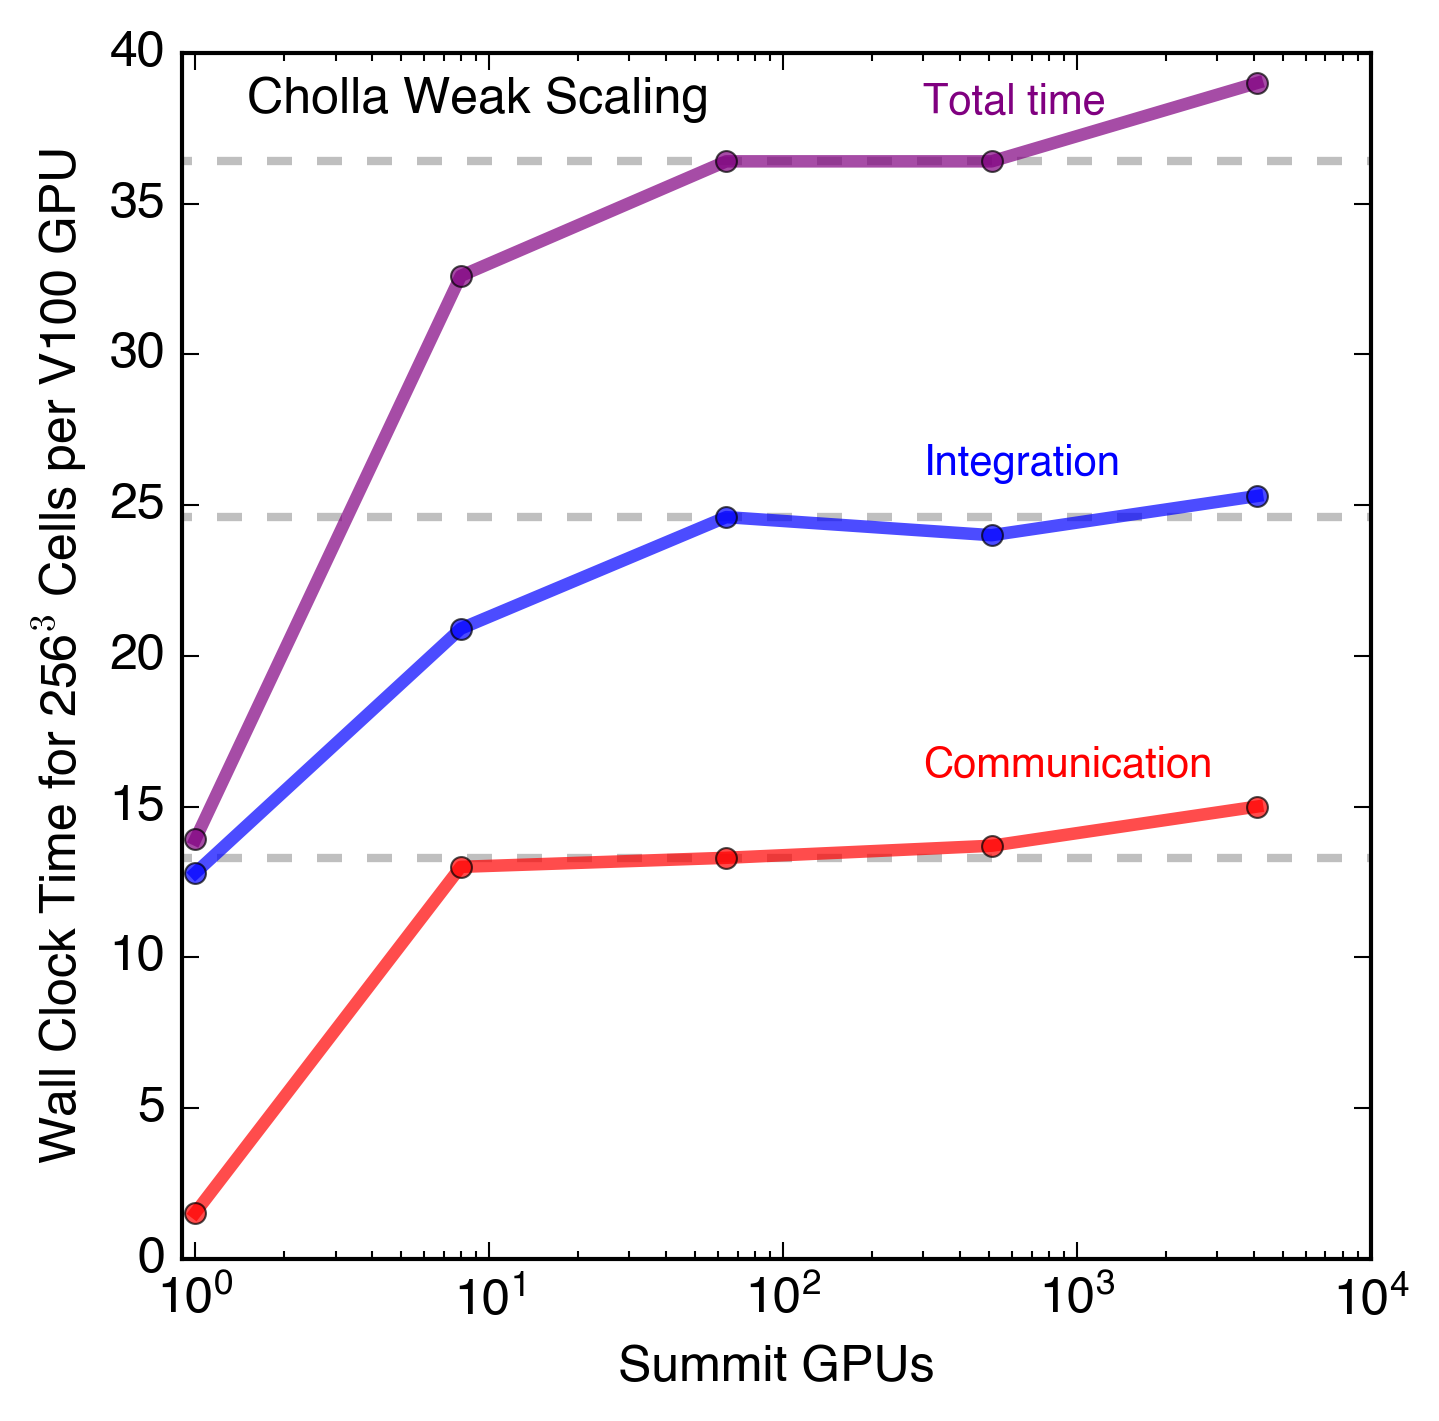
\includegraphics[width=4.52in, height=3.08in, keepaspectratio=true]{../scaling/weak_scaling_adiabatic.png}
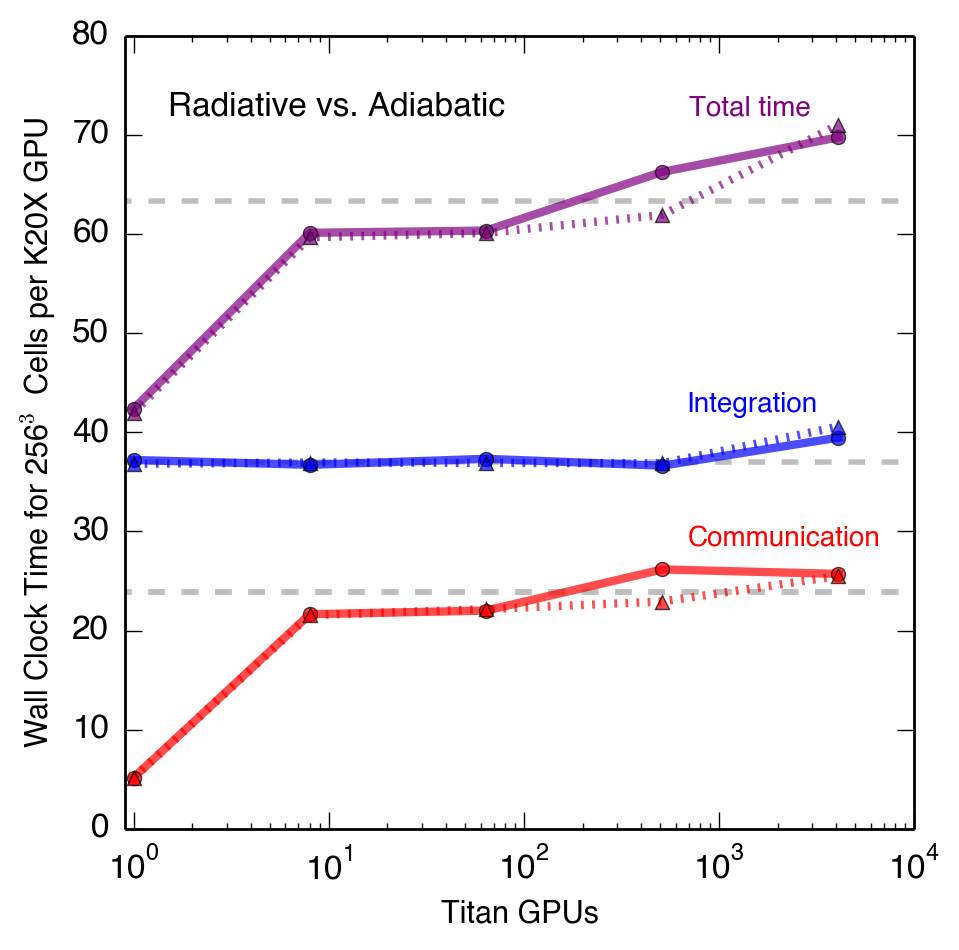
\includegraphics[width=4.52in, height=3.08in, keepaspectratio=true]{weak_scaling_radiative.png}
\caption{Weak scaling tests with {\tt Cholla}. Shown is the wall clock execution time for an acoustic wave propagation test simulation when the number of cells per GPU is kept fixed at $256^3$. The left panel shows tests performed on Summit, while the right panel comparing adiabatic hydrodynamics to radiative hydrodynamics was performed on Titan.
The code exhibits excellent weak scaling over three orders of magnitude on Summit, up to the maximum 4096 GPUs available for testing as of June 1. The total simulation (purple), hydro algorithm (blue), and communications plus boundary conditions (red) timings are shown separately for comparison. In each case, the ideal scaling would be constant (gray dashed lines). Our novel GPU hardware-accelerated implementation of radiative cooling (right panel) allows for radiative simulations (dotted lines, triangles) to match otherwise identical 
adiabatic simulations (solid lines; circles) in computational efficiency and weak scaling, as tested to 4096 GPUs. (Note that the tests for the left and right panels were run for a different total amount of time - our tests have shown that {\tt Cholla} runs $3.8\times$ faster {\it per GPU} on Summit vs. Titan.)}
\label{fig:weak_scaling}
\end{figure}

We have implemented a novel GPU-accelerated radiative cooling scheme into {\tt Cholla} that uses the texture memory on the GPU
to perform linear interpolation on pre-computed cooling tables as a function of the gas density and temperature. The right
panel of Figure~\ref{fig:weak_scaling} compares the timing of adiabatic (solid) and radiatively-cooling (dotted) sound wave
propagation tests using $256^3$ cells per GPU on the Titan XK7 system, and demonstrates that the weak scaling performance
of the {\tt Cholla} code is nearly identical with or without radiative cooling. These tests are very similar to the calculations that will be performed 
in our turbulent CGM simulations, giving us additional confidence in our estimated run time for the petascale simulations that require optically-thin radiative cooling.


\vspace{-.25in}
\subsection{Developmental Work}
\vspace{-.2in}

%For the computational approach above, describe what, if any, development work has been carried out to date, especially on the architecture of the requested resource. Describe what development work will be executed, and when, during the proposed INCITE campaign, and an estimate of the computational resources required for this work.  If applicable, identify the milestones and production simulations in Section 2.3.i that are dependent on the developmental work and provide a plan for validating this developmental work.
Most of the developmental work for this program has either already been completed, or will be complete by the start of 2019. However, we highlight below some of the additional physics modules in {\tt Cholla} that will be used in this work, particularly those that we may improve over the coming months.

\vspace{-.2in}
\subsubsection{Cooling: COMPLETED}
\vspace{-.25in}


Since the publication of \cite{Schneider15}, a primary developmental task for the {\tt Cholla} codebase was
 the now-completed implementation of a model for optically-thin cooling. This task formed much of the motivation for
our DD Project AST119 granted in January 2016. This developmental work is complete and is
described in \cite{Schneider17}. Algorithmically, energy losses due to radiative cooling are precomputed using the
{\tt Cloudy} code \cite{Ferland13} assuming solar metallicity and a photoionizing
cosmic UV background. The cooling rates are stored in a two-dimensional table,
and interpolated as a function of gas density and temperature. This interpolation 
is GPU-accelerated by storing the table in texture memory on the GPU, which allows
for interpolation to be performed natively by the hardware using the CUDA {\tt cudaTextureObject\_t} and {\tt tex2D} capabilities.
We also use timestep subcycling combined with a forward-Euler integration to account for short cooling timescales in high density gas and radiative shocks. Even when several subcycles are required, this method of calculating radiative cooling remarkably adds negligible computational cost, allowing the superior
weak scaling of {\tt Cholla} to be maintained (see Figure \ref{fig:weak_scaling}).

\vspace{-.2in}
\subsubsection{Turbulence Generator: In Progress}
\vspace{-.25in}

A turbulence generator has already been built for {\tt Cholla}, however, we do have plans to improve it for this project. The current model imposes a series of ``kicks" to the velocities of each cell, with the energy injection rate normalized to offset energy losses due to radiative cooling. The velocity perturbations are applied over the course of a single time step at discreet intervals, typically 1/10th of the turbulent crossing time, $\Delta t = 0.1 L / c_s$. In addition to the kick model, this work will make use of a constant energy injection mode of turbulence driving that is currently under construction. In the constant energy model, kinetic energy is re-added to the grid at the end of each time step in an amount that exactly balances the global radiative losses. Co-PI Fielding has experience implementing this sort of turbulence generator in {\tt Athena}, a very similar fixed-grid code, and will be implementing it in {\tt Cholla} in the coming months.

\vspace{-.2in}
\subsubsection{Conduction: In Progress, Supplemental}
\vspace{-.25in}

While not strictly required for the simulations outlined in this proposal, conduction is an additional physical process that may have an effect on the physical state of gas in the circumgalactic medium. We have begun development work on a conduction module for {\tt Cholla}, which will allow us to further explore the nature of thermal instability in the CGM. This development is being done in conjunction with our current INCITE project (AST125), and as such, will be complete by the end of 2018. We expect to use conduction in a subset of the parameter study simulations at low pressure where the resolution requirements are not as stringent. (If the effects are substantial, we may apply for additional INCITE time in the future, but we believe the results from the convergence study with thermal instability alone will be an important step forward in this field, and a fully-resolved study with conduction is beyond the scope of this proposal.)

\vspace{-.3in}
\section{REFERENCES}
\vspace{-.3in}

%References are optional and may be structured in accordance with any style. They {\bf \em {do not}} count toward the 15-page limit.
%\vspace{-.15in}

{\footnotesize
\bibliographystyle{usrt}
\renewcommand{\section}[2]{}
\begin{thebibliography}{500}
\bibitem{Schneider15} Schneider, E. and Robertson, B., ``{\tt Cholla}: A New Massively Parallel Hydrodynamics Code for Astrophysical Simulation'', {\em ApJS}, {\bf 217}, 24 (2015).
\bibitem{Tumlinson17} Tumlinson, J., Peeples, M.~S., \& Werk, J.~K.\ 2017,  ``The Circumgalactic Medium", {\em ARAA}, 55, 389 
\bibitem{Putman12} Putman, M.~E., Peek, J.~E.~G., \& Joung, M.~R.\ 2012,  ``Gaseous Galaxy Halos", {\em ARAA}, 50, 491 
\bibitem{White78} White, S.~D.~M., \& Rees, M.~J.\ 1978,  ``Core condensation in heavy halos - A two-stage theory for galaxy formation and clustering", {\em MNRAS}, 183, 341 
\bibitem{Fielding17} Fielding, D., et al. ``The Impact of Star Formation Feedback on the Circumgalactic Medium." {\em MNRAS}, {\bf 466}, 3810 (2017).
\bibitem{Bregman07} Bregman, J.~N.\ 2007,  ``The Search for the Missing Baryons at Low Redshift", {\em ARAA}, 45, 221
\bibitem{Keres09} Kere{\v s}, D., Katz, N., Fardal, M., Dav{\'e}, R., \& Weinberg, D.~H.\ 2009,  ``Galaxies in a simulated {$\Lambda$}CDM Universe - I. Cold mode and hot cores", {\em MNRAS}, 395, 160
\bibitem{Wakker2009}  Wakker, B.~P.,  \& Savage, B.~D.\ 2009,  "The Relationship Between Intergalactic H I/O VI and Nearby ($z < 0.017$) Galaxies.``, {\rm ApJS}, 182, 378
\bibitem{Rigby02} Rigby, J.~R., Charlton, J.~C., \& Churchill, C.~W.\ 2002,  ``The Population of Weak Mg II Absorbers. II. The Properties of Single-Cloud Systems", {\em ApJ}, 565, 743 
\bibitem{Tumlinson13} Tumlinson, J., et al.\ 2013,  ``The COS-Halos Survey: Rationale, Design, and a Census of Circumgalactic Neutral Hydrogen", {\em ApJ}, 777, 59 
\bibitem{Werk14} Werk, J.~K., et al.\ 2014,  ``The COS-Halos Survey: Physical Conditions and Baryonic Mass in the Low-redshift Circumgalactic Medium", {\em ApJ}, 792, 8 
\bibitem{Lau16} Lau, M.~W., Prochaska, J.~X., \& Hennawi, J.~F.\ 2016,  ``Quasars Probing Quasars. VIII. The Physical Properties of the Cool Circumgalactic Medium Surrounding z \~{} 2 - 3 Massive Galaxies Hosting Quasars", {\em ApJS}, 226, 25 
\bibitem{Chen2009} Chen, H.-W., \& Mulchaey, J.~S.\ 2009,  ``Probing The Intergalactic Medium-Galaxy Connection At $z < 0.5$. I. A Galaxy Survey In Qso Fields And A Galaxy-Absorber Cross-Correlation Study", {\em ApJ}, 701, 1219 
\bibitem{Prochaska2011} Prochaska, J.~X., Weiner, B., Chen, H.-W., Mulchaey, J., \& Cooksey, K.\ 2011,  ``Probing the Intergalactic Medium/Galaxy Connection. V. On the Origin of Ly{$\alpha$} and O VI Absorption at $z < 0.2$", {\em ApJ}, 740, 91 
\bibitem{Hummels2013} Hummels, C.~B., Bryan, G.~L., Smith, B.~D., \& Turk, M.~J.\ 2013,  ``Constraints on hydrodynamical subgrid models from quasar absorption line studies of the simulated circumgalactic medium", {\em MNRAS}, 430, 1548 
\bibitem{Tumlinson11} Tumlinson, J. et al. ``The Large, Oxygen-Rich Halos of Star-Forming Galaxies Are a Major Reservoir of Galactic Metal'', {\em Science}, {\bf 344}, 948 (2011)
\bibitem{Bordoloi14} Bordoloi, R. et al. ``The COS-Dwarfs Survey: The Carbon Reservoir around Sub-L* Galaxies'', {\em ApJ}, {\bf 796}, 136 (2014)
\bibitem{Borthakur15} Borthakur, S. et al. ``Connection between the Circumgalactic Medium and the Interstellar Medium of Galaxies: Results from the COS-GASS Survey'', {\em ApJ}, {\bf 813}, 46 (2015)
\bibitem{Thom12} Thom, C. et al. ``Not Dead Yet: Cool Circumgalactic Gas in the Halos of Early-type Galaxies'', {\em ApJ}, {\bf 758}, 41 (2012)
\bibitem{Rauch02} Rauch, M. et al.  ``Small-Scale Structure at High Redshift. IV. Low-Ionization Gas Intersecting Three Lines of Sight to Q2237+0305'' {\em ApJ}, {\bf 576}, 54 (2002)
\bibitem{Churchill03} Churchill, C. et al. ``The Spatial, Ionization, and Kinematic Conditions of the z=1.39 Damped Ly? Absorber in Q0957+561A, B'' {\em ApJ}, {\bf 593}, 203 (2003)
\bibitem{Lopez18} Lopez, S. et al. ``A clumpy and anisotropic galaxy halo at redshift 1 from gravitational-arc tomography'', {\em Nature}, {\bf 554}, 493 (2018) 
\bibitem{McCourt18} McCourt, M., et al. ``A characteristic scale for cold gas." {\em MNRAS}, {\bf 473}, 5407 (2018).
\bibitem{McQuinnWerk} McQuinn, M. \& Werk, J. ``Implications of the Large O VI Columns around Low-redshift L ? Galaxies'', {\em ApJ}, {\bf 852}, 33, (2018)
\bibitem{SpringelHernquist} Springel, V. \& Hernquist, L. ``Cosmological smoothed particle hydrodynamics simulations: a hybrid multiphase model for star formation'', {\em MNRAS}, {\bf 339}, 289 (2003)
\bibitem{Schneider17} Schneider, E. and Robertson, B., ``Hydrodynamical Coupling of Mass and Momentum in Multiphase Galactic Winds'', {\em ApJ}, {\bf 834}, 144 (2017).
\bibitem{Schneider18a} Schneider, E. and Robertson, B., `Introducing `CGOLS: The Cholla Galactic OutfLow Simulation Suite,'' {\em Astrophysical Journal}  {\bf in press} (2018) \\
\bibitem{Schneider18b} Schneider, E., et al. ``Production of Cool Gas in Thermally-Driven Outflows,'' {\em Astrophysical Journal} {\bf in press} (2018) \\
\bibitem{Godunov59} Godunov, S., ``A Difference Scheme for Numerical Solution of Discontinuous Solution of Hydrodynamic Equations.'' {\em Math. Sbornik}, {\bf 47}, 271 (1959)
\bibitem{Ferland13} Ferland, G., et al. ``The 2013 Release of Cloudy.'' {\em RMAA}, {\bf 49}, 137 (2013)



\bibitem{Nelson+16} Nelson, D. et al. ``Zooming in on accretion - I. The structure of halo gas'', {\em MNRAS}, {\bf 460}, 2881 (2016)
\vspace{-.09in}
\end{thebibliography}
}



\end{document}
